\subsection{Design concept}
\label{sec:design}

In this section, we present the basic design concept of FDPS. We first
present the abstract view of calculation codes for particle-based
simulations on distributed-memory parallel computers, and then
describe how such abstraction is realized in FDPS.


\subsubsection{Abstract view of particle-based simulation codes}
\label{sec:view}

In a particle-based simulation code that uses the space decomposition on
distributed-memory parallel computers, the calculation proceeds in the
following steps:
\begin{enumerate}

\item The computational domain is divided into subdomains, and each
  subdomain is assigned to one MPI process. This step is usually
  called domain decomposition. Here, minimization of inter-process
  communication and a good load balance among  processes should be
  achieved.
 \label{proc:decompose}

\item Particles are exchanged among  processes, so that each
  process owns particles in its subdomain. In this paper we call this
  step particle exchange.
  \label{proc:exchange}

\item Each process collects the information necessary to calculate the
  interactions on its particles. We call this step
  interaction-information exchange.
  \label{proc:interactionexchange}

\item Each process calculates interactions between particles in its
  subdomain. We call this step interaction calculation.
  \label{proc:interaction}

\item The data for each particle are updated using the calculated
  interactions. This part is done without inter-process communication.
   \label{proc:local}
\end{enumerate}

Steps \ref{proc:decompose}, \ref{proc:exchange}, and
\ref{proc:interactionexchange} involve parallelization and
inter-process communications. FDPS provides library functions to
perform these parts. Therefore, users of FDPS do not have to write the
parallelization and/or inter-process communication part of their own
code at all.

Step \ref{proc:interaction} does not involve inter-process
communication. However, this step are necessary to perform the actual
calculation of interactions between two particles.  Users of FDPS
should write a simple interaction kernel. The actual interaction
calculation using the tree algorithm or neighbor search is done in the
FDPS side.

%However, it requires either the use of tree algorithm
%or FMM (long-range interactions), or neighbor search (short-range
%interactions), and actual calculation of interactions between
%particles.  Users of FDPS should write a simple interaction kernel,
%and actual interaction calculation using the tree algorithm or
%neighbor search is done in the FDPS side.

Step \ref{proc:local} involves neither inter-process communication nor
interaction calculation. Users of FDPS should and can write their own
program for this part. 

%In the following we describe briefly how FDPS provide the application
%program interface (API) for steps \ref{proc:decompose} through.  for
%arbitrary systems of particles.

%% JM 2016081418

FDPS can be used to implement particle-based simulation codes for
initial value problems which can be expressed as the following
ordinary differential equations:

\begin{eqnarray}
%\begin{align}
  \frac{d\myvec{u}_i}{dt} = \myvec{g}\left(\sum_j^N \myvec{f}
  (\myvec{u}_i, \myvec{u}_j), \myvec{u}_i\right). \label{eq:geq}
%\end{align}
\end{eqnarray}
  
Here, $N$ is the number of particles in the system, $\myvec{u}_i$ is
a vector which represents the physical quantities of  particle $i$, 
$\myvec{f}$ is a function which describes
the contribution of particle $j$ to the time derivative of
physical quantities of particle $i$, and $\myvec{g}$ is a function
which converts the sum of the contributions to the actual time
derivative. In the case of gravitational $N$-body
simulation, $\myvec{u}_i$ contains position, velocity, mass, and other
parameters of  particle $i$, $\myvec{f}$ is the gravitational force
from particle $j$ to particle $i$, and 
$\myvec{g}$ gives velocity as the time derivative of  position and
calculated acceleration as the time derivative of velocity.

Hereafter, we call a particle that receives the interaction
``$i$-particle'', and a particle exerting that interaction
``$j$-particle''. The actual contents of vector $\myvec{u}_i$ and the
functional forms of $\myvec{f}$ and $\myvec{g}$ depend on the physical
system and numerical scheme used.

In equation (\ref{eq:geq}) we included only the pairwise interactions,
because usually the calculation cost of the pairwise interaction is
the highest even when many-body interaction is important. For example,
angle and torsion of bonding force in simulation of organic molecules
can be done in the user code, with small additional computing cost.


\subsubsection{Design concept of FDPS}
\label{sec:concept}

In this section, we describe how the abstract view presented in the
previous section is actually expressed in the FDPS API (application
programming interface).  The API of FDPS is defined as a set of
template library functions in C++ language.


\begin{figure}
  \begin{center}
    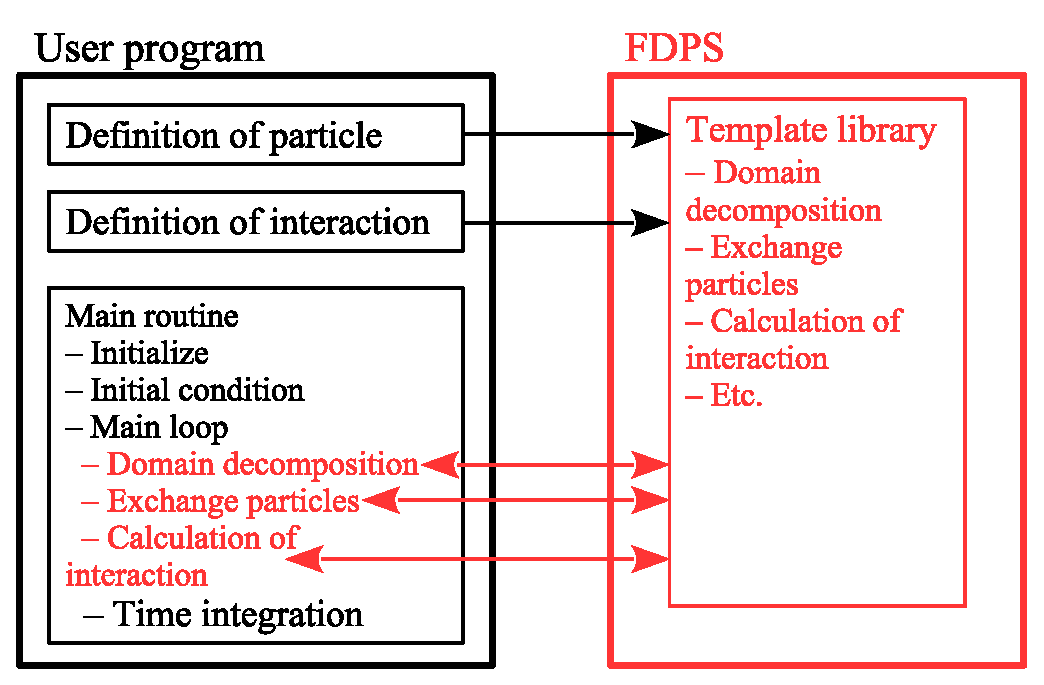
\includegraphics[width=8cm]{figure/concept.eps}
  \end{center}
  \caption{The basic concept of FDPS. The user program gives the
    definitions of particle and interaction to FDPS, and calls FDPS
    APIs.}
  \label{fig:concept}
\end{figure}


Figure~\ref{fig:concept} shows how a user program and FDPS library
functions interact.  The user program gives the definition of a
particle $\myvec{u}_i$ and particle-particle interaction $\myvec{f}$
to FDPS at the compile time. They are written in the standard C++
language. Thus, the user program [at least the main() function]
currently should be written in C++\footnote{We will investigate a
  possible way to use APIs of FDPS from programs written in Fortran.}.

%% 02081511

The user program first does the initialization of FDPS library. When
the user program is compiled for the MPI environment, the
initialization of MPI communication is done in the FDPS initialization
function.  The setup of the initial condition is done in the user
program.  It is possible to use file input function defined in FDPS.
In the main integration loop, domain decomposition, particle exchange,
interaction information exchange and force calculation are all done
through library calls to FDPS.  The time integration of the physical
quantities of particles using the calculated interaction, is done
within the user program.

%% A user of FDPS can develop the simulation code in the following three
%% steps:
%% \begin{enumerate}
%% \item Define the data structure for $\myvec{u}_i$, as a class in the
%%   C++ language.
%% \item Define the function $\myvec{f}$. It receives arrays of
%%   $i$-particles and $j$-particles, and calculates and accumulates
%%   $\myvec{f}$ on $i$-particles.

%%   %It should be a function object in C++ language\footnote{A function
%%   %pointer of C language can be operable.}, which receives arrays of
%%   %  $i$-particles and $j$-particles, and calculates and accumulates
%%   %  $\myvec{f}$ on $i$-particles.
  
%% \item Write the user program using the data class and functions
%%   provided by FDPS. Currently, the user program should also be written
%%   in C++.
%% \end{enumerate}

Note that it is possible to implement multi-stage integration schemes
such as the Runge-Kutta schemes using FDPS. FDPS can evaluate the
right-hand side of equation (\ref{eq:geq}) for a given set of
$\myvec{u}_i$. Therefore, the derivative calculation for intermediate
steps can be done by passing $\myvec{u}_i$ containing appropriate
values.

The parallelization using MPI is completely taken care by FDPS, and
the use of OpenMP is also taken care by FDPS for the interaction
calculation. In order to achieve high performance, the interaction
calculation should make efficient use of the cache memory and SIMD
units. In FDPS, this is done by requiring an interaction calculation
function to calculate the interactions between multiple $i$- and
$j$-particles. In this way, the amount of memory access is
significantly reduced, since single $j$-particle is used to calculate
the interaction on multiple $i$-particles ($i$-particles are also in
the cache memory). To make the efficient use of the SIMD execution
units, currently the user should write the interaction calculation
loop so that the compiler can generate SIMD instructions. Of course,
the use of libraries optimized for specific architectures
\citep{2006NewA...12..169N, 2012NewA...17...82T, 2013NewA...19...74T}
would guarantee very high performance.

It is also possible to use GPUs and other accelerators for the
interaction calculation. In order to reduce the communication
overhead, so-called ``multiwalk'' method \citet{hamada2009novel}, is
implemented. Thus, interaction calculation kernels for accelerators
should take multiple sets of the pair of $i$- and $j$-particles. The
performance of this version will be discussed elsewhere.

\begin{figure}
  \begin{center}
    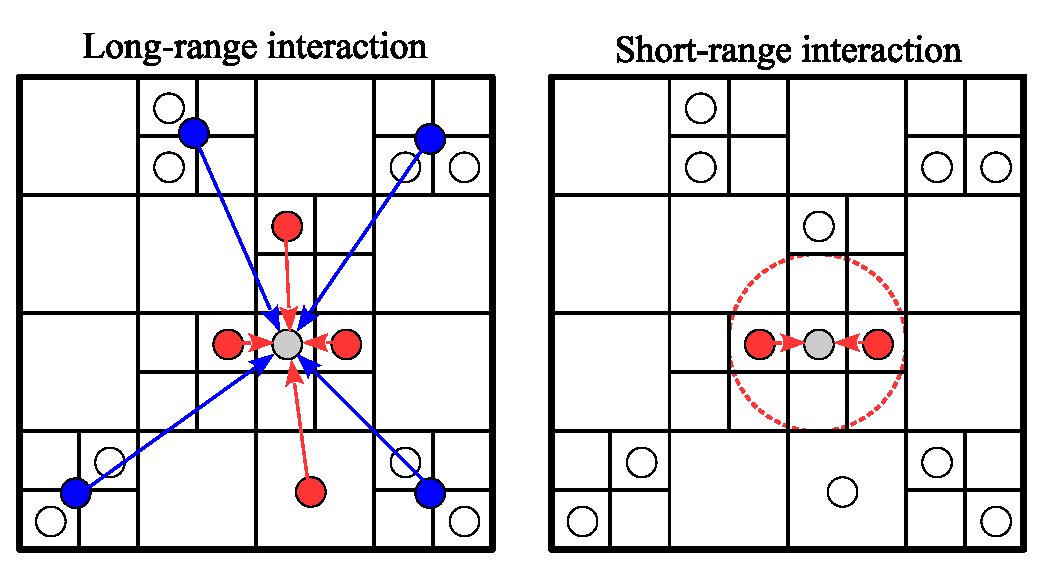
\includegraphics[width=8cm]{figure/force_type.eps}
  \end{center}
  \caption{Long-range interaction (left) and short-range interaction
    (right). Gray, red, and blue points are $i$-particles,
    $j$-particles, and superparticles, respectively.}
  \label{fig:forcetype}
\end{figure}

As stated earlier, FDPS performs the neighbor search if the interaction
is of short-range nature. If the long-range interaction is used,
currently FDPS uses the Barnes-Hut tree algorithm. In other words,
within FDPS, the distinction between the long-range and short-range
interactions is not a physical one but an operational one. If we want
to apply the treecode, it is a long-range interaction. Otherwise, it is
a short-range interaction.  Thus, we can use the simple tree
algorithm for pure $1/r$ gravity and the TreePM scheme
\citep{1995ApJS...98..355X, 2000ApJS..128..561B, 2002JApA...23..185B,
  2004NewA....9..111D, 2005MNRAS.364.1105S, 2005PASJ...57..849Y,
  2009PASJ...61.1319I, Ishiyama:2012:PAN:2388996.2389003} for the
periodic boundary.


Figure~\ref{fig:forcetype} illustrates the long-range and short-range
interactions and how they are calculated in FDPS.

For  long-range interactions, Barnes-Hut algorithm is used. Thus, the
interactions from a group of distant particles are replaced by that of
a superparticle, and  equation~(\ref{eq:geq}) is modified to 
%\begin{align}
\begin{eqnarray}
  \frac{d\myvec{u}_i}{dt} = \myvec{g}\left( \sum_j^{N_{\mathrm{J},i}}
  \myvec{f}(\myvec{u}_i,\myvec{u}_j) + \sum_{j'}^{N_{\mathrm{S},i}}
  \myvec{f'}(\myvec{u}_i,\myvec{u'}_{j'}), \myvec{u}_i
  \right), \label{eq:geqL}
%\end{align}
\end{eqnarray}
where $N_{\mathrm{J},i}$ and $N_{\mathrm{S},i}$ are, the number of
$j$-particles and superparticles for which we apply multipole-like
expansion, the vector $\myvec{u'}_{j'}$ is the physical quantity
vector of a superparticle, and the function $\myvec{f'}$ indicates the
interaction exerted on particle $i$ by the superparticle $j'$. In
simulations with a large number of particles $N$, $N_{\mathrm{J},i}$
and $N_{\mathrm{S},i}$ are many orders of magnitude smaller than $N$.
A user need to give functions to construct superparticles from
particles and to calculate the interaction from superparticles. Since
the most common use of the long-range interaction is for $1/r$
potential, FDPS includes standard implementation of these functions
for $1/r$ potential for  up to the quadrupole moment.




% LocalWords:  FDPS subdomains subdomain MPI parallelization dt discretized API
% LocalWords:  APIs timestep Runge Kutta OpenMP SIMD vectorization AoS SoA PME
% LocalWords:  multipole FFT TreePM parallelized superparticles superparticle
% LocalWords:  quadrupole
